
\usetikzlibrary{matrix}
\usetikzlibrary{shapes}
\usetikzlibrary{positioning}

\begin{adjustbox}{width=0.6\textwidth}
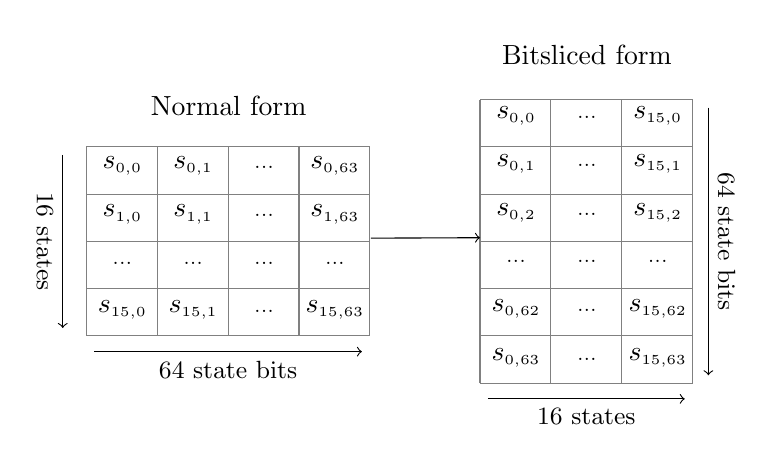
\begin{tikzpicture}
[
     block/.style={rectangle, fill=none, text width=7em, text centered, minimum height=2em},
]

\draw[->] (0.1,-.2) -- (3.5,-.2) node[below,midway] {\small 64 state bits};
\draw[->] (-0.3,2.3) -- (-.3,.1) node[below,midway,sloped] {\small 16 states};
\begin{scope}
\draw[xstep=0.9cm,ystep=0.6,color=gray] (0,0) grid (3.6,2.4);
\matrix[matrix of nodes,
inner sep=0pt,
anchor=south west,
nodes={inner sep=0pt,text width=.9cm,align=center,minimum height=.6cm}
](m1){
$s_{\scriptscriptstyle 0,0}$ & $s_{\scriptscriptstyle 0,1}$ & $\scriptstyle \ldots$ & $s_{\scriptscriptstyle 0,63}$  \\
$s_{\scriptscriptstyle 1,0}$ & $s_{\scriptscriptstyle 1,1}$ & $\scriptstyle \ldots$ & $s_{\scriptscriptstyle 1,63}$  \\
$\scriptstyle \ldots$  & $\scriptstyle \ldots$&$\scriptstyle \ldots$ &$\scriptstyle \ldots$  \\
$s_{\scriptscriptstyle 15,0}$ & $s_{\scriptscriptstyle 15,1}$ & $\scriptstyle \ldots$ & $s_{\scriptscriptstyle 15,63}$  \\
};
 \end{scope}

\node [block,above=.1cm of m1] (text1) {Normal form};

 \begin{scope}[xshift=5cm]
 \draw[->] (0.1,-.8) -- (2.6,-.8) node[below,midway] {\small 16 states};
 \draw[->] (2.9,2.9) -- (2.9,-0.5) node[above,midway,sloped] {\small 64 state bits};
\draw[xstep=0.9cm,ystep=0.6,color=gray] (0,-0.6) grid (2.7,3);
\matrix[matrix of nodes,
inner sep=0pt,
anchor=south west,
nodes={inner sep=0pt,text width=.9cm,align=center,minimum height=.6cm}
] at (0,-0.6)(m2){
$s_{\scriptscriptstyle 0,0}$ &  $\scriptstyle \ldots$ & $s_{\scriptscriptstyle 15,0}$  \\
$s_{\scriptscriptstyle 0,1}$ &  $\scriptstyle \ldots$ & $s_{\scriptscriptstyle 15,1}$  \\
$s_{\scriptscriptstyle 0,2}$ &  $\scriptstyle \ldots$ & $s_{\scriptscriptstyle 15,2}$  \\
$\scriptstyle \ldots$  & $\scriptstyle \ldots$ &$\scriptstyle \ldots$  \\
$s_{\scriptscriptstyle 0,62}$ &  $\scriptstyle \ldots$ & $s_{\scriptscriptstyle 15,62}$  \\
$s_{\scriptscriptstyle 0,63}$ &  $\scriptstyle \ldots$ & $s_{\scriptscriptstyle 15,63}$  \\
};
 \end{scope}
 
 \node [block,above=.1cm of m2] (text1) {Bitsliced form};

\draw[->] (m1) -- (m2);

\end{tikzpicture}
\end{adjustbox}